%%%%%%%%%%%%%%%%%%%%%%%%%%%%%%%%%%%%%%%%%
% University Assignment Title Page 
% LaTeX Template
% Version 1.0 (27/12/12)
%
% This template has been downloaded from:
% http://www.LaTeXTemplates.com
%
% Original author:
% WikiBooks (http://en.wikibooks.org/wiki/LaTeX/Title_Creation)
%
% License:
% CC BY-NC-SA 3.0 (http://creativecommons.org/licenses/by-nc-sa/3.0/)
% 
% Instructions for using this template:
% This title page is capable of being compiled as is. This is not useful for 
% including it in another document. To do this, you have two options: 
%
% 1) Copy/paste everything between \begin{document} and \end{document} 
% starting at \begin{titlepage} and paste this into another LaTeX file where you 
% want your title page.
% OR
% 2) Remove everything outside the \begin{titlepage} and \end{titlepage} and 
% move this file to the same directory as the LaTeX file you wish to add it to. 
% Then add \input{./title_page_1.tex} to your LaTeX file where you want your
% title page.
%
%%%%%%%%%%%%%%%%%%%%%%%%%%%%%%%%%%%%%%%%%
%\title{Title page with logo}
%----------------------------------------------------------------------------------------
%	PACKAGES AND OTHER DOCUMENT CONFIGURATIONS
%----------------------------------------------------------------------------------------

\documentclass[12pt]{article}
% \usepackage[english]{babel}
% \usepackage[utf8x]{inputenc}
\usepackage{amsmath}
\usepackage{graphicx}
\usepackage{listings}
\usepackage{biblatex}
\bibliography{references.bib}
% \usepackage[colorinlistoftodos]{todonotes}
\newtheorem{theorem}{Theorem}


\textheight=250truemm \textwidth=160truemm 
\hoffset=-10truemm \voffset=-30truemm

\begin{document}

\begin{titlepage}

\newcommand{\HRule}{\rule{\linewidth}{0.5mm}} % Defines a new command for the horizontal lines, change thickness here

\center % Center everything on the page
 
%----------------------------------------------------------------------------------------
%	HEADING SECTIONS
%----------------------------------------------------------------------------------------
\vspace*{0.5cm}
\textsc{\LARGE Ukrainian Catholic University}\\[1cm] % Name of your university/college
\textsc{\Large  Faculty of Applied Sciences}\\[0.5cm] % Major heading such as course name
\textsc{\large Data Science Master Programme}\\[0.5cm] % Minor heading such as course title

%----------------------------------------------------------------------------------------
%	TITLE SECTION
%----------------------------------------------------------------------------------------
\vspace*{1.5cm}

\HRule \\[0.4cm]
{ \huge \bfseries Interpretability libraries comparison}\\[10pt]
{\Large \bfseries Responsible Data Science project report}\\[0.4cm] % Title of your document
\HRule \\[1cm]
 
%----------------------------------------------------------------------------------------
%	AUTHOR SECTION
%----------------------------------------------------------------------------------------
\vspace*{2.5cm}

\Large \emph{Authors:}\\
Konstantyn  \textsc{Ovchynnikov}\\
Dmitrii \textsc{Glushko}\\
Yuriy \textsc{Lizak}\\
Olena \textsc{Shevchenko}\\[1cm] % Your name

%----------------------------------------------------------------------------------------
%	DATE SECTION
%----------------------------------------------------------------------------------------
\vspace*{0.5cm}
{\large \today}\\[0.5cm] % Date, change the \today to a set date if you want to be precise

%----------------------------------------------------------------------------------------
%	LOGO SECTION
%----------------------------------------------------------------------------------------


\includegraphics[height=5cm]{UCU-Apps.png}\\[0.5cm] % Include a department/university logo - this will require the graphicx package
 
%----------------------------------------------------------------------------------------
% Fill the rest of the page with whitespace

\end{titlepage}
\vspace*{0.8cm}
\section{Introduction}
Today we are surrounded by applications of Machine learning. It helps us quickly write letters, corrects grammar, recommends movies and products, unlocks our phone. We are getting used to it; some of us do not really care how such algorithms make decisions, others do. Though some applications are harmless, meaning a mistake will not have serious consequences (e.g., a movie recommender system), others might heavily influence our life by making a mistake (e.g., autonomous driving). Generally, we might want to know 'what was predicted?' and 'why the prediction was made.' To answer the second question, the interpretability comes in handy. \\
According to \textit{Miller}\cite{Miller}: \textbf{Interpretability is the degree to which a human can understand the cause of a decision.}
Another definition\cite{NIPS2016_6300} is \textbf{Interpretability is the degree to which a human can consistently predict the model’s result.} So the interpretability is a measure of an answer to 'why' question, is it only?  Various teams around the world work on the understanding of model decision making to make black box models more transparent. Different algorithms had been developed and open sourced. In this work, we want to explore the functionality of popular libraries and analyze their interpretability power.

\section{Related work}
The easiest way to achieve interpretability is to use only a subset of algorithms that create interpretable models. Linear regression, logistic regression, and the decision tree are commonly used interpretable models.\cite{molnar2019}
Such models are well described in terms of their explanatory power, so we will not pay additional attention to these models. \\
With the increasing popularity of deep learning, various teams work of mechanisms to achieve model agnostic interpretability\cite{ribeiro2016model}.The team from the University of Washington \textit{Ribeiro et al.}\cite{RibeiroSG16}  presented the local interpretable model-agnostic explanations (LIME) that work with any classifier. 

\section{Problems}
We want to investigate the interpretability systems based on two different tasks - Credit Scoring and Image Classification. Link to the Github project\cite{Project}

\subsection{Credit Scoring}
A credit score is a numerical expression based on a level analysis of a person's credit files, to represent the creditworthiness of an individual. Traditionally, a credit score was primarily based on credit report information typically sourced from credit bureaus. \\
\textbf{About the Dataset:} Lending Club Dataset \\
Lending Club is a US peer-to-peer lending company, headquartered in San Francisco, California. Lending Club is the world's largest peer-to-peer lending platform. The company states that \$15.98 billion in loans had been originated through its platform up to 31 December 2015.


\section{Model-agnostic systems}
In their work \textit{Ribeiro et al.}\cite{ribeiro2016model} describes desirable properties of model-agnostic explanation systems. Authors point out three such features:
\begin{itemize}
    \item Model flexibility -  can work with both linear models and deep networks
    \item Explanation flexibility - not limited to a certain form of explanation
    \item Representation flexibility - should be able to use a different feature representation as the model being explained. 
\end{itemize}

\subsection{SHAP}
SHAP (SHapley Additive exPlanations) presented by \textit{Lundberg and Lee} \cite{SHAP} at NIPS 2017 as a unified way to interpret model predictions. 
SHAP is a unified approach to explain the output of any machine learning model. SHAP connects game theory with local explanations, representing the only possible consistent and locally accurate additive feature attribution method based on expectations. \\
We will use Python Shap library on two tasks (credit scoring, image classification), to understand It's abilities, advantages and disadvantages.\\
Shap has model flexibility - this library can work with Tree ensembles, Linear models, and Deep Learning models also. By the time, Shap is one of the most famous libraries, it has good explanation flexibility. There is an ability to look at single observation (or multiple) to understand, which features influenced the result in which way (higher/lower). \\
Shap API is straightforward. \\
\begin{lstlisting}
----------------------------------------------------
# Explainer can work with any Python model
explainer = shap.KernelExplainer(model.predict_proba, subsample)
# Extracting shap values matrix
shap_values = explainer.shap_values(subsample)
\end{lstlisting}
Representation flexibility is important part of this research, so we was trying to use all visualization abilities of the library to get better understanding of prediction results and features influence.\\
First plot was used to get feature influence and which range of values created this influence. At this plot we can see, for example,  how higher number of delinquincies impacted the model.\\
\\
\\

\begin{figure}[!htb]
\centering
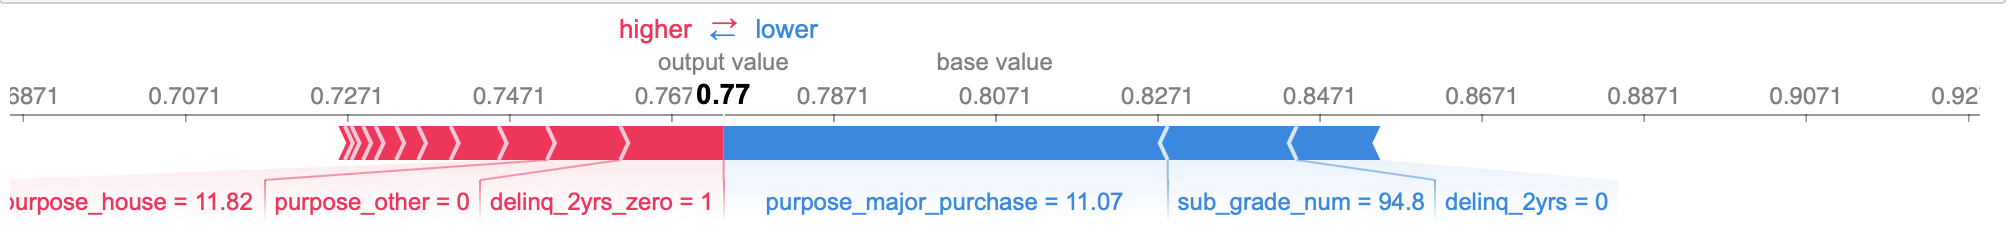
\includegraphics[height=5cm]{shap_ex1.png}\\[0.5cm] 
\caption{Summary plot by all features in credit scoring task. }
\end{figure}

After looking at big picture, library gives the ability to look at single observation output and features influence.
\begin{figure}[!htb]

\centering
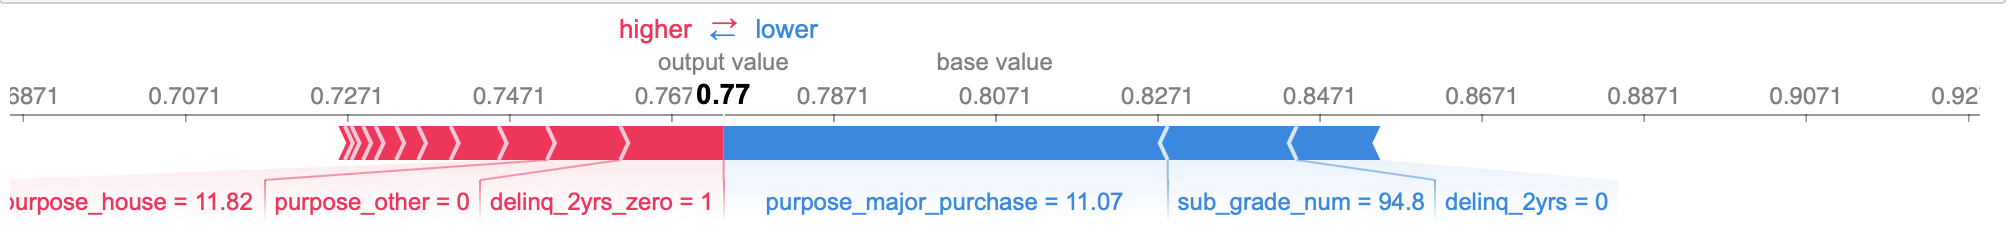
\includegraphics[height=2cm]{shap_ex2.png}\\[0.5cm] 
\caption{Example of single observation explanation.}
\end{figure}
\\
Library has ability to build dependence plots. For example we can look at the most influencial features.

\begin{figure}[!htb]
\centering
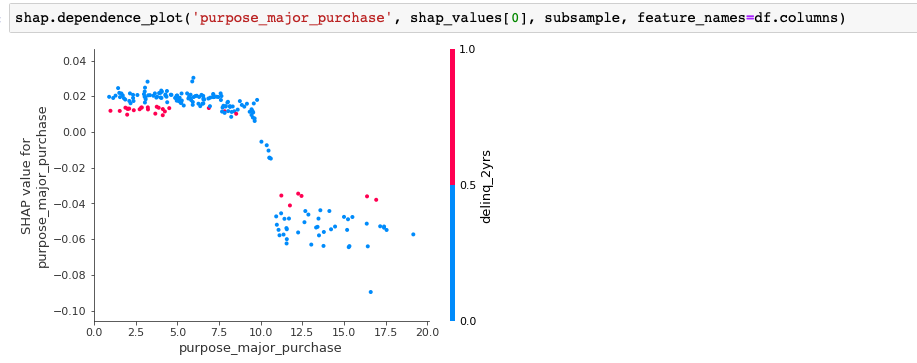
\includegraphics[height=5cm]{shap_ex3.png}\\[0.5cm] 
\caption{Example of dependence plot for scoring task.}
\end{figure}

\begin{figure}[!htb]
\centering
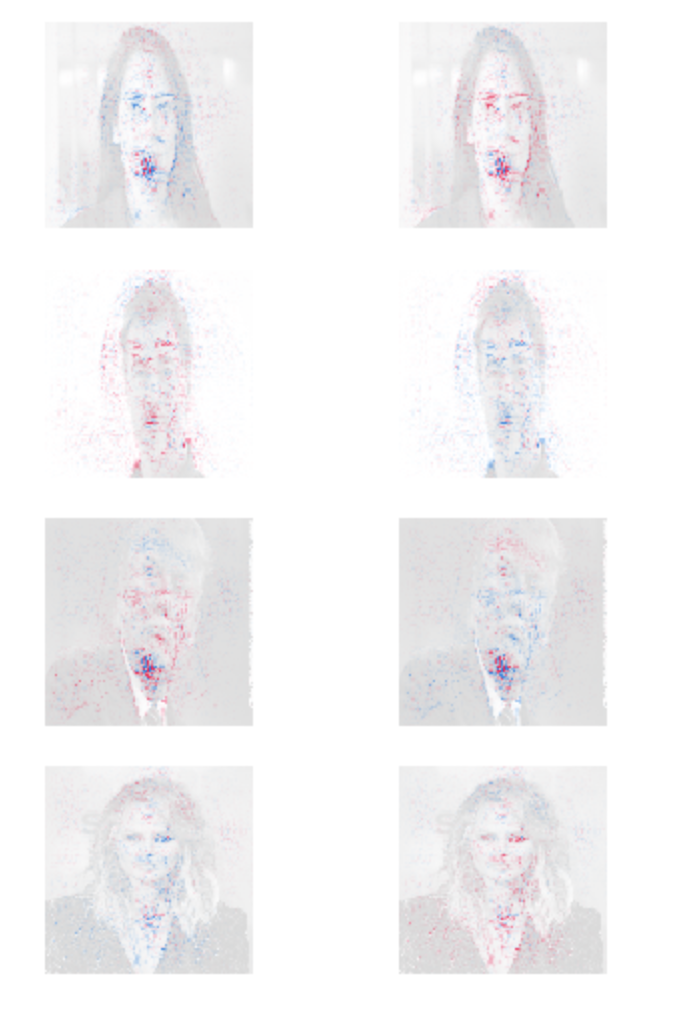
\includegraphics[height=5cm]{shap_ex4.png}\\[0.5cm] 
\caption{Deep learning model feature maps. Explains visually which features was used to make predictions.}
\end{figure}
\newpage
\subsection{SKATER}
Skater is an open-source python library for model interpretation. The project started at the beginning of 2017 and is currently under active development in the beta phase. \\
Skater supports interpretation on two levels: global - using information from the whole dataset, local - using information about one prediction to approximate functions based on inputs and outputs. Global interpretation is supported by the next algorithms:
\begin{itemize}
    \item Model agnostic Feature Importance
    \item Model agnostic Partial Dependence Plots
    \item Scalable Bayesian Rule Lists
    \item Tree Surrogates
\end{itemize}
Local interpretation is realized using:
\begin{itemize}
    \item Local Interpretable Model Explanation (LIME)
    \item Layer-wise Relevance Propagation (e-LRP): image
    \item Integrated Gradient: image and text
    \item Scalable Bayesian Rule Lists
    \item Tree Surrogates
\end{itemize}
The framework supports the most popular Python libraries. It can work with models from scikit-learn, XGBoost, Keras, Tensorflow. \\
In this project, Skater was applied to interpret Gender Classification model based on the VGGNet Architecture. 3 methods were used to explain the model:
\begin{itemize}
    \item Epsilon-LRP
    \item Integrated Gradient
    \item Occlusion
\end{itemize}

Layer-wise Relevance Propagation is a method that identifies important pixels by running a backward pass in the neural network. It starts from the output and weight the neurons that contribute the most. How to implement it can be found in \cite{LRP_Implementation}. \\

Integrated Gradients is a method to find the relation between a deep model's prediction and its features. Like in our example it is a relation to the pixels. The method is based on the paper \cite{Integrated_Gradients}. \\

Occlusion as an algorithm that computes direct relevance of the input features by removing or masking them, running a forward pass and measuring the difference between old and new output. Explained in detail by \cite{Occlusion}. \\

Corresponding code of using Skater on VGGNet can be found in \textit{interpretability/skater\textunderscore library.ipynb} ipython notebook. \\


\begin{figure}[!htb]
\centering
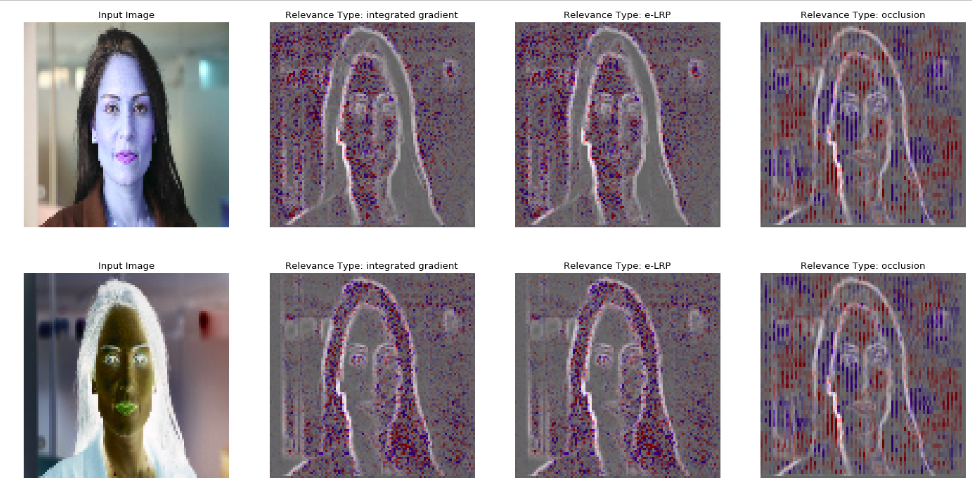
\includegraphics[height=7cm]{skater_ex1.png}\\[0.5cm] 
\caption{Local VGGNet model interpretability with Skater}
\end{figure}


All three methods are trying to find out the importance of the pixels for the specific prediction.
Looking at the result with the woman example we can see that the current model has a strong relation between hair pixels and the prediction. Both Integrated Gradient and Epsilon-LRP show almost the same result. In contrast, looking at the occlusion method, it is hard to get a good interpretation of the model. So using Skater with local interpretation approaches it is easy to add some interpretability to CNN networks even having few examples.

\section{Conclusions}
We've tried several libraries with two different (deep learning, tree) models. Most of them had model flexibility so we can work with both models. 
Shap library has more flexibility in representation features and visualization techniques. It is more supported by the community, too. It's a disadvantage - library works slow. \\
Skater has also flexibility in the available functionality. The framework has different interpretation algorithms and methods available for different models including deep neural networks like CNN. But it's still in the beta phase and the functionality sometimes looks raw. However, it is in active development.
Summarising the frameworks we analyzed, there are a lot of different algorithms and methods that are already implemented and work nice with existing libraries like sci-kit-learn, Keras, Tensorflow making live of the data scientist easier and giving time to stay focused on the domain part of the problem. But from another point of view, all these techniques are pretty generic so far and can't cover all the possible cases, meaning that the data scientist can always encounter the situation where the specific solution must be applied with using the specific domain knowledge.

\section{Peer Review}
Work done:
\begin{itemize}
    \item Dmitrii Glushko: Gender Classification model preparation, Skater library analysis and report section
    \item Konstantyn Ovchynnikov: Credit Scoring model preparation, SHAP library analysis and report section
    \item Yuriy Lizak: LIME library analysis
    \item Olena Shevchenko: report skeleton, introduction, related work
\end{itemize}

\newpage
\printbibliography
\end{document}